\documentclass[fleqn]{jbook}
\usepackage{physpub}
\usepackage[dvipdfm]{graphicx}
\usepackage{amsmath}
\usepackage{amscd}
\usepackage{amssymb}
\usepackage{wrapfloat}
\usepackage{subfigure}
\setlength{\columnsep}{3zw}
%\setlength{\columnseprule}{0.4pt}
\if01 % by Murase
  % \thesection は physpub で \hspace{-1zw} に上書きされている。
  % 本来の \thesection を使いたければ、\Thesection に退避されている物を使用。
  \renewcommand{\theequation}{\thesection.\arabic{equation}}
  \renewcommand{\thefigure}{\thesection.\arabic{figure}}
  \renewcommand{\thetable}{\thesection.\arabic{table}}
  \numberwithin{equation}{section}
  \numberwithin{figure}{section}
  \numberwithin{table}{section}
\fi
%\renewcommand{\figurename}{Fig}
\usepackage[usenames]{color}
%\title{平成16年度院試解答例 物理学}

\begin{document}

%===============================================================================
\begin{question}{第1問}{}
%問題はM.Yが入力しました

幅$a$、深さ$-V_0 (<0)$の一次元井戸型ポテンシャル$V(x)$を考える (図\iref{2004phy1-0})。質量$m$の粒子が、$x=-\infty$から波数$k$の平面波$e^{ikx}$で入射すると、その一部は反射し、一部は透過する。このとき、$x<-a/2$と$x>a/2$における波動関数を、それぞれ$\psi=e^{ikx}+Re^{-ikx}, \psi=Te^{ikx}$とし、また$-a/2\le x\le a/2$における波動関数を$\psi=\alpha e^{ikx}+\beta e^{-ikx}$として、以下の設問に答えよ。但し、$\hbar=h/(2\pi)$($h$はプランク定数)とする。

\begin{figure}[htbp]
\begin{center}
%\includegraphics[scale=0.4]{2004phy1-0.eps}
\includegraphics[width=6cm]{2004phys1_0.eps}
\caption{}
\eqname{2004phy1-0}
\end{center}
\end{figure}

\begin{enumerate}
\item 入射波、反射波、透過波に対するフラックス(確率密度の流れ)を、$\hbar, m, k, R,T$を用いて表せ。また$T$と$R$の関係式を与えよ。
\item $T=|T|e^{i\theta}$と書くとき、位相$\theta$が現れる物理的理由を簡潔に述べよ。
\item $p$を$\hbar,m,k,V_0$を用いて表せ。
\item $T$を以下の式のように表すとき、$A$と$B$を$k$と$p$を用いて表せ。
$$
T=\frac{e^{-ika}}{A\cos(pa)-iB\sin(pa)}
$$

\item 入射した波が反射を全く受けない(完全透過する)為の$k$が満たすべき条件を求めよ。また、完全透過がおこる物理的理由を簡潔に述べよ。

\item $|T|^2$を$k$の関数として図示せよ。
\end{enumerate}
\end{question}



%===============================================================================
\begin{answer}{第1問}{}
\begin{enumerate}
\item
\begin{figure}[htbp]
 \begin{center}
\resizebox{!}{5cm}{%WinTpicVersion3.08
\unitlength 0.1in
\begin{picture}( 42.3000, 27.3000)(  3.7000,-28.0000)
% LINE 2 0 3 0
% 2 400 1600 400 1600
% 
\special{pn 8}%
\special{pa 400 1600}%
\special{pa 400 1600}%
\special{fp}%
% VECTOR 2 0 3 0
% 4 400 1600 4600 1600 2400 2800 2400 200
% 
\special{pn 8}%
\special{pa 400 1600}%
\special{pa 4600 1600}%
\special{fp}%
\special{sh 1}%
\special{pa 4600 1600}%
\special{pa 4534 1580}%
\special{pa 4548 1600}%
\special{pa 4534 1620}%
\special{pa 4600 1600}%
\special{fp}%
\special{pa 2400 2800}%
\special{pa 2400 200}%
\special{fp}%
\special{sh 1}%
\special{pa 2400 200}%
\special{pa 2380 268}%
\special{pa 2400 254}%
\special{pa 2420 268}%
\special{pa 2400 200}%
\special{fp}%
% LINE 2 0 3 0
% 6 1600 1600 1600 2600 1600 2600 3200 2600 3200 2600 3200 1600
% 
\special{pn 8}%
\special{pa 1600 1600}%
\special{pa 1600 2600}%
\special{fp}%
\special{pa 1600 2600}%
\special{pa 3200 2600}%
\special{fp}%
\special{pa 3200 2600}%
\special{pa 3200 1600}%
\special{fp}%
% VECTOR 2 0 3 0
% 6 400 1400 1200 1400 1200 1800 400 1800 3400 1400 4200 1400
% 
\special{pn 8}%
\special{pa 400 1400}%
\special{pa 1200 1400}%
\special{fp}%
\special{sh 1}%
\special{pa 1200 1400}%
\special{pa 1134 1380}%
\special{pa 1148 1400}%
\special{pa 1134 1420}%
\special{pa 1200 1400}%
\special{fp}%
\special{pa 1200 1800}%
\special{pa 400 1800}%
\special{fp}%
\special{sh 1}%
\special{pa 400 1800}%
\special{pa 468 1820}%
\special{pa 454 1800}%
\special{pa 468 1780}%
\special{pa 400 1800}%
\special{fp}%
\special{pa 3400 1400}%
\special{pa 4200 1400}%
\special{fp}%
\special{sh 1}%
\special{pa 4200 1400}%
\special{pa 4134 1380}%
\special{pa 4148 1400}%
\special{pa 4134 1420}%
\special{pa 4200 1400}%
\special{fp}%
% STR 2 0 3 0
% 3 4600 1610 4600 1710 1 0
% $x$
\put(46.0000,-17.1000){\makebox(0,0)[lt]{$x$}}%
% STR 2 0 3 0
% 3 3250 1570 3250 1670 1 0
% $\frac{a}{2}$
\put(32.5000,-16.7000){\makebox(0,0)[lt]{$\frac{a}{2}$}}%
% STR 2 0 3 0
% 3 1540 1570 1540 1670 4 0
% $\frac{a}{2}$
\put(15.4000,-16.7000){\makebox(0,0)[rt]{$\frac{a}{2}$}}%
% STR 2 0 3 0
% 3 2440 1460 2440 1560 2 0
% $0$
\put(24.4000,-15.6000){\makebox(0,0)[lb]{$0$}}%
% STR 2 0 3 0
% 3 2440 2540 2440 2640 1 0
% $V_0$
\put(24.4000,-26.4000){\makebox(0,0)[lt]{$V_0$}}%
% STR 2 0 3 0
% 3 2470 140 2470 240 2 0
% $V(x)$
\put(24.7000,-2.4000){\makebox(0,0)[lb]{$V(x)$}}%
% STR 2 0 3 0
% 3 670 1240 670 1340 2 0
% $e^{ikx}$
\put(6.7000,-13.4000){\makebox(0,0)[lb]{$e^{ikx}$}}%
% STR 2 0 3 0
% 3 3600 1240 3600 1340 2 0
% $Te^{ikx}$
\put(36.0000,-13.4000){\makebox(0,0)[lb]{$Te^{ikx}$}}%
% STR 2 0 3 0
% 3 600 1790 600 1890 1 0
% $Re^{-ikx}$
\put(6.0000,-18.9000){\makebox(0,0)[lt]{$Re^{-ikx}$}}%
\end{picture}%
}
 \end{center}
\caption{井戸型ポテンシャル}
\eqname{fig:potential}
\end{figure}

Fluxは次のように定義される.
\begin{equation}\
 \vec{J}=Re\left(\psi^* \frac{\hbar}{im}\nabla \psi\right)=\frac{\hbar}{2mi}\left[\psi^* \nabla \psi-\psi \nabla\psi^*\right] \eqname{eq:1}
\end{equation}
今の場合$x$成分を考えると,
\paragraph{$x<-a/2$のとき}
\begin{align}
 J_{x,\text{I}}&= Re\left[(e^{-ikx}+R^* e^{ikx})\frac{\hbar}{im}ik(e^{ikx}-Re^{-ikx})\right]\nonumber  \\
& \,\,\,\,(\text{I}=(-\infty ,-a/2))\nonumber\\
&=\frac{\hbar k}{m}Re\left[\left\{ 1-|R|^2+(R^* e^{2ikx}-Re^{-2ikx})\right\}\right]\nonumber\\
&=\frac{\hbar k}{m}(1-|R|^2) \eqname{eq:2}
\end{align}
\paragraph{$-a/2 <x <a/2$のとき}
\begin{equation}
 J_{x,\text{II}}=\frac{\hbar k}{m}(|\alpha|^2 -|\beta|^2)\,\,\,\,(\text{II}=(-a/2,a,2)) \eqname{eq:3}
\end{equation}
\paragraph{$x>a/2$のとき}
\begin{equation}
 J_{x,\text{III}}=\frac{\hbar k}{m}|T|^2\,\,\,\,\,(\text{III}=(a/2,\infty))\eqname{eq:4}
\end{equation}
よって入射波,反射波,透過波に対するフラックスはそれぞれ
\begin{align}
 J_{\text{in}}= \frac{\hbar k}{m},\,\,\,\, J_{\text{re}}=\frac{\hbar k}{m}|R|^2,\,\,\,\, J_{\text{tr}}=\frac{\hbar k}{m}|T|^2 \eqname{eq:5}
\end{align}
フラックスの保存により
\begin{align*}
 \frac{\hbar k}{m}(1-|R|^2)&=\frac{\hbar k}{m}(|\alpha|^2-|\beta|^2)=\frac{\hbar k}{m}|T|^2\\
∴\,\, 1&=|R|^2+|T|^2
\end{align*}
が成り立つ.
\item
入射波は$x=\pm a/2$で一部が反射し,残りが透過する.$a=a/2$で反射
した波は再び$x=- a/2$で反射波と透過波に分かれ,さらに$x=-a/2$で反射し
た波は再び$x=a/2$で反射波と透過波に分かれる.このように
$-a/2 < x <a/2$
の両端では何度も波が反射と透過を繰り返す.従って,最終的に$a/2<x$の領域
に出てくる波$T e^{ikx}$はそれらの波の重ね合わせになっていると考えら
れる.この結果,透過波の位相が入射波の位相からずれる.また,同様
の理由で$R e^{-ikx}$の位相も入射波の位相からずれているはずである.
\item
Schr\"{o}dinger eq.は
\begin{equation}
 \left[  -\frac{\hbar^2}{2m}\bigtriangleup +V(x)\right]\psi (x)=E \psi (x)\eqname{eq:6}
\end{equation}
である.\\
井戸の外側($|x|>a/2$)では$V(x)=0$であって
$\psi(x)=Te^{ikx}(\text{or},e^{ikx}+Re^{-ikx})$を式\eqhref{eq:6})に代入すると\\
\begin{equation}
 \frac{\hbar^2}{2m}k^2=E \eqname{eq:7}
\end{equation}
を得る.\\
他方,井戸の内側($|x|< a/2$)のときは$V(x)=-V_0$であり$\psi (x)=\alpha e^{ikx}+\beta
e^{-ikx}$を式(\eqhref{eq:6})に代入して
\begin{equation}
 \frac{\hbar^2 p^2}{2m}=V_0 +E \eqname{eq:8}
\end{equation}
を得る.式~(\eqhref{eq:7}),~(\eqhref{eq:8})から
\begin{equation}
 p=\sqrt{k^2+\frac{2mV_0}{\hbar^2}} \eqname{eq:9}
\end{equation}
となる.
\item
波動関数は$x=\pm a/2$で滑らかに接続される.\\
\begin{align}
&(x=a/2=:b)\nonumber\\ 
& \left\{ 
\begin{array}[tb]{rl}
Te^{ikb} & =\alpha e^{ikb}+\beta e^{-ikb}\\
ikTe^{ikb}& = ip(\alpha e^{ikb}-\beta e^{-ikb})
\end{array}
\right.\eqname{eq:11}
\end{align}


\begin{align}
&(x=-b) \nonumber\\
 & \left\{
 \begin{array}{rl}
 e^{-ikb}+Re^{ikb}&=\alpha e^{-ipb}+\beta e^{ipb} \\
 ik(e^{-ikb}-Re^{ikb})&= ip(\alpha e^{-ipb}-\beta e^{ipb})
 \end{array}
 \right.\eqname{eq:10}
\end{align}

 式~(\eqhref{eq:11})より
\begin{equation}
 \left(
\begin{array}{c}
  \alpha\\ \beta
\end{array}
 \right) =\frac{Te^{ikb}}{2p}
\left[
\begin{array}{c}
 (p+k)e^{-ipb}\\(p-k)e^{ipb}
\end{array}
\right]\eqname{eq:12}
\end{equation}
これを~式(\eqhref{eq:10})に代入し,$R$を消去すると
\begin{equation}
 T= \frac{e^{-ika}}{\cos(pa)-i\frac{p^2+k^2}{2kp}\sin(pa)}\eqname{eq:13}
\end{equation}
が得られた.
\item
保存の式($|R|^2+|T|^2=1$)より,完全透過するのは$|T|^2=1$の時である.
式~(\eqhref{eq:13})より
\begin{align}
|T|^2&=\frac{1}{\cos^2(pa)+\left(\frac{p^2+k^2}{2kp}\right)^2\sin^2(pa)}=1 \nonumber\\
∴&(p^2-k^2)^2 \sin^2(pa)=0 \eqname{eq:14}
\end{align}
$V_0\neq 0$であるから$p\neq k$.よって
\begin{equation}
 pa=n\pi \Leftrightarrow (ka)^2=(n\pi)^2-\frac{2ma^2 V_0}{\hbar^2}\,\,\,\,(n\in \textbf{Z}_{>0})\eqname{eq:15}
\end{equation}
但し最後の変形には式~(\eqhref{eq:9})を用いた.\\
\begin{figure}[h]
\begin{center}
 %WinTpicVersion3.08
\unitlength 0.1in
\begin{picture}( 32.0000, 28.0000)(  4.0000,-34.0000)
% LINE 2 0 3 0
% 2 400 1600 400 1600
% 
\special{pn 8}%
\special{pa 400 1600}%
\special{pa 400 1600}%
\special{fp}%
% VECTOR 2 0 3 0
% 4 400 1600 3600 1600 1800 2600 1800 600
% 
\special{pn 8}%
\special{pa 400 1600}%
\special{pa 3600 1600}%
\special{fp}%
\special{sh 1}%
\special{pa 3600 1600}%
\special{pa 3534 1580}%
\special{pa 3548 1600}%
\special{pa 3534 1620}%
\special{pa 3600 1600}%
\special{fp}%
\special{pa 1800 2600}%
\special{pa 1800 600}%
\special{fp}%
\special{sh 1}%
\special{pa 1800 600}%
\special{pa 1780 668}%
\special{pa 1800 654}%
\special{pa 1820 668}%
\special{pa 1800 600}%
\special{fp}%
% ELLIPSE 1 0 3 0
% 4 1800 3200 3800 1650 2800 1850 800 1850
% 
\special{pn 13}%
\special{ar 1800 3200 2000 1550  4.1912668 5.2335111}%
% ELLIPSE 1 0 3 0
% 4 1800 400 4000 2020 800 1850 2800 1850
% 
\special{pn 13}%
\special{ar 1800 400 2200 1620  1.1008710 2.0407217}%
% LINE 2 0 3 0
% 6 800 1600 800 2800 800 2800 2800 2800 2800 2800 2800 1600
% 
\special{pn 8}%
\special{pa 800 1600}%
\special{pa 800 2800}%
\special{fp}%
\special{pa 800 2800}%
\special{pa 2800 2800}%
\special{fp}%
\special{pa 2800 2800}%
\special{pa 2800 1600}%
\special{fp}%
% LINE 2 0 3 0
% 2 1800 1600 1800 3400
% 
\special{pn 8}%
\special{pa 1800 1600}%
\special{pa 1800 3400}%
\special{fp}%
% ELLIPSE 1 0 3 0
% 4 1300 3200 2300 4200 1800 2400 800 2400
% 
\special{pn 13}%
\special{ar 1300 3200 1000 1000  4.1537897 5.2709883}%
% ELLIPSE 1 0 3 0
% 4 2300 3200 3300 2200 2800 2200 1800 2400
% 
\special{pn 13}%
\special{ar 2300 3200 1000 1000  4.1537897 5.1760366}%
% ELLIPSE 1 0 3 0
% 4 1300 1400 2700 2400 800 2330 1800 2330
% 
\special{pn 13}%
\special{ar 1300 1400 1400 1000  1.2041373 1.9374554}%
% ELLIPSE 1 0 3 0
% 4 2300 1400 3500 2410 1800 2320 2800 2320
% 
\special{pn 13}%
\special{ar 2300 1400 1200 1010  1.1417589 1.9998338}%
% VECTOR 2 0 3 0
% 4 1800 1410 2800 1410 1800 1410 800 1410
% 
\special{pn 8}%
\special{pa 1800 1410}%
\special{pa 2800 1410}%
\special{fp}%
\special{sh 1}%
\special{pa 2800 1410}%
\special{pa 2734 1390}%
\special{pa 2748 1410}%
\special{pa 2734 1430}%
\special{pa 2800 1410}%
\special{fp}%
\special{pa 1800 1410}%
\special{pa 800 1410}%
\special{fp}%
\special{sh 1}%
\special{pa 800 1410}%
\special{pa 868 1430}%
\special{pa 854 1410}%
\special{pa 868 1390}%
\special{pa 800 1410}%
\special{fp}%
% STR 2 0 3 0
% 3 1980 1280 1980 1380 2 0
% $a$
\put(19.8000,-13.8000){\makebox(0,0)[lb]{$a$}}%
% STR 2 0 3 0
% 3 3580 1600 3580 1700 1 0
% $x$
\put(35.8000,-17.0000){\makebox(0,0)[lt]{$x$}}%
% STR 2 0 3 0
% 3 1830 2790 1830 2890 1 0
% $-V_0$
\put(18.3000,-28.9000){\makebox(0,0)[lt]{$-V_0$}}%
\end{picture}%

\end{center}
\caption{干渉現象}
\eqname{fig:teizaiha} 
\end{figure}
ここで求めた条件は一種の干渉現象と考えることができる.井戸型のポテンシャ
ルの幅$a$が半波長の整数倍を含むとき,定在波が生じる(図~\iref{fig:teizaiha}).
定在波が生じると,波動関数は常に$x=\pm a/2$で節になる.
よって,入射波は反射することなく井戸を越えることが出来る.
定在波が生じる条件は
\begin{equation}
 a=\frac{1}{2}\cdot\frac{2\pi}{p}\times n\,\,\,\,(n \in \textbf{Z}_{>0}) \eqname{eq:25}
\end{equation}
と現されるが,これは確かに式~(\eqhref{eq:15})に等しい.
\item
\[
 |T(k)|^2=\left[ 1+ \frac{1}{4}\left(\frac{2mV_0}{\hbar^2}\right)^2 \frac{\sin^2(pa)}{p^2k^2}\right]^{-1}
\]
を図示すると図~\iref{fig:touka}のようになる.透過係数はだんだんと増してい
く下縁の包絡線と$1$の間を振動する.
\begin{figure}[htbp]
 \begin{center}
\resizebox{7cm}{!}{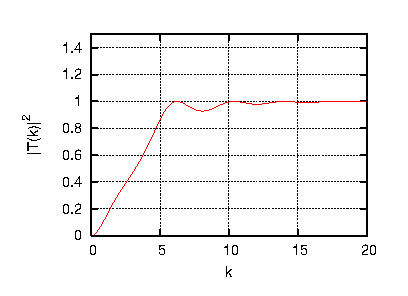
\includegraphics{2004phy1-3.eps}}
 \end{center}
\caption{$|T(k)|^2$の振る舞い}
\eqname{fig:touka}
\end{figure}
\end{enumerate}
\end{answer}
\end{document}
